% A schematic diagram showing the shape of the feature map as it passes through the network.

\documentclass{standalone}
\usepackage{tikz}
\usetikzlibrary{shapes.geometric, arrows.meta, positioning, calc, fit}

% Styles - blocks
\tikzstyle{block} = [rectangle, draw, text centered, minimum width=2cm, minimum height=1cm, fill=white]
\tikzstyle{attention} = [circle, draw, text centered, minimum size=1cm, fill=orange!20]
\tikzstyle{concatmerge} = [circle, draw, text centered, minimum size=0.05cm, font=\tiny]

% arrows
\tikzstyle{conv} = [thick, ->, >=stealth, black]
\tikzstyle{pool} = [thick, ->, >=stealth, green]
\tikzstyle{up}   = [thick, ->, >=stealth, orange]
\tikzstyle{skip} = [thick, dashed, ->, >=stealth, gray]
\tikzstyle{gate} = [thick, ->, >=stealth, blue]
\tikzstyle{merge} = [thick, ->, >=stealth, red]


\begin{document}
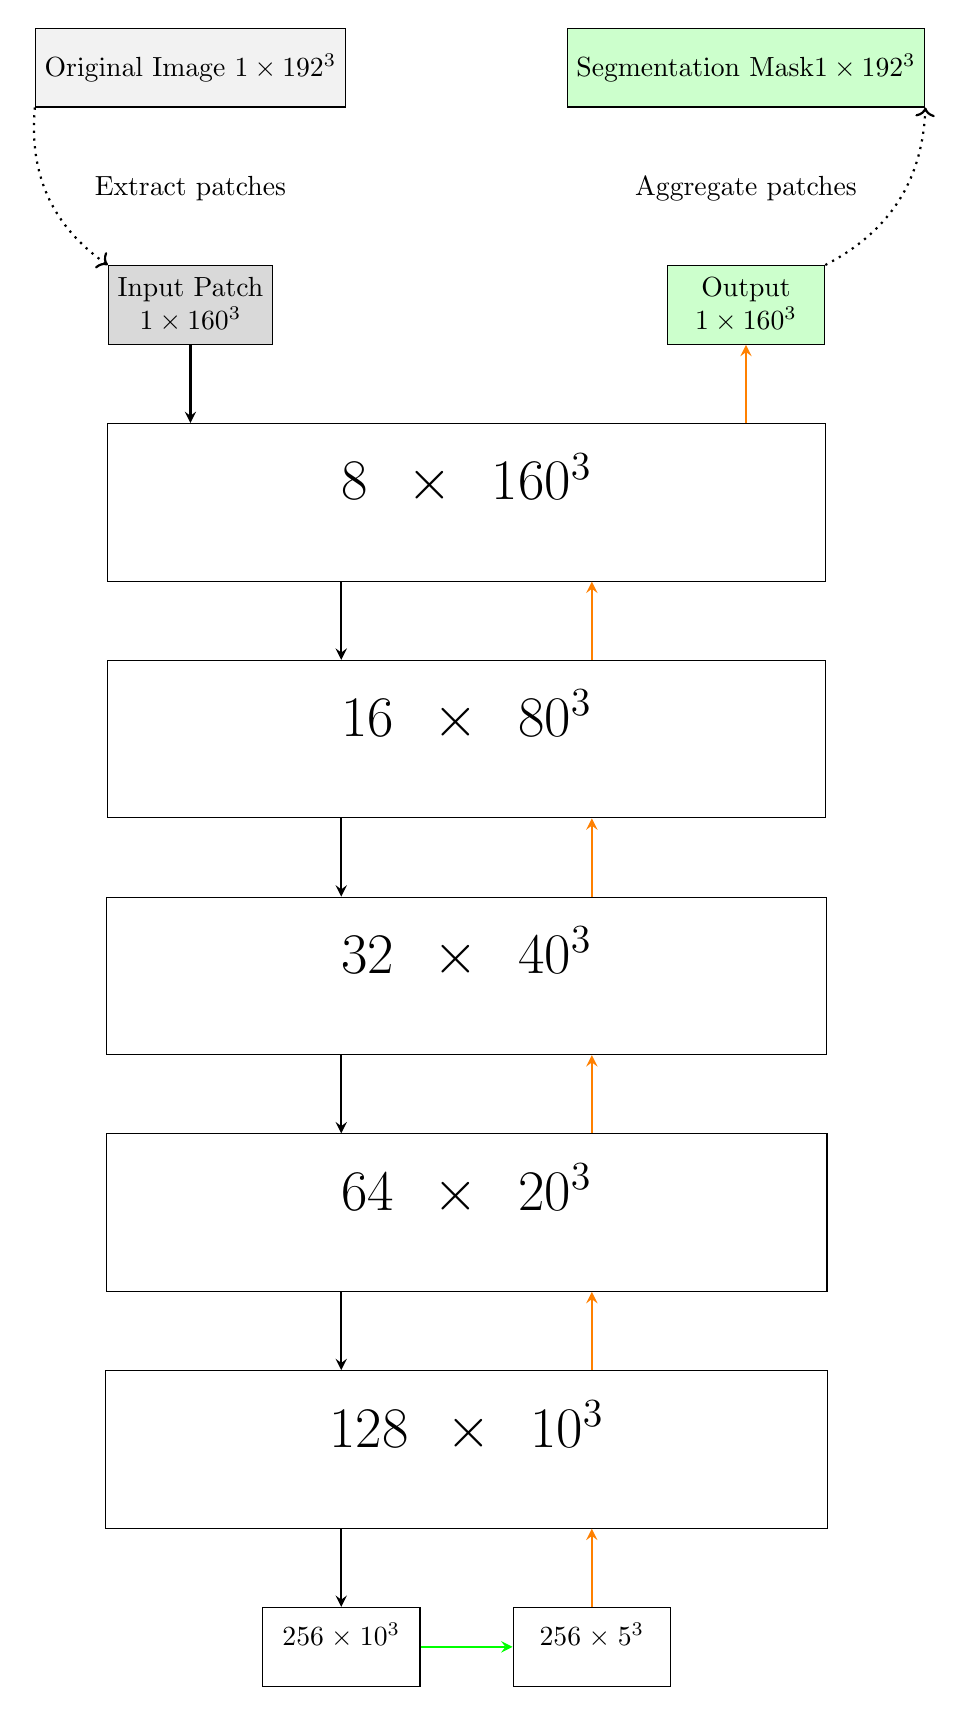
\begin{tikzpicture}[node distance=1.8cm and 0.5cm]

	% Inputs
	\node (input_full) [block, fill=gray!10] {Original Image $1\times192^3$};
	\node (input_patch) [block, below=2cm of input_full, fill=gray!30, align=center] {Input Patch\\$1\times160^3$};

	% Outputs
	\node (output_patch) [block, right=5cm of input_patch, fill=green!20, align=center] {Output\\$1\times160^3$};
	\node (output_full) [block, fill=green!20, above=2cm of output_patch] {Segmentation Mask$1\times192^3$};

	% Labels
	\node (extraction) [below=0.75cm of input_full, align=center] {Extract patches};
	\node (stitching) [below=0.75cm of output_full, align=center] {Aggregate patches};

	% Blocks
	\node[draw, fit={([yshift=-1cm]input_patch.south west) ([yshift=-3cm]output_patch.south east)}, inner sep=0pt, align=center] (block0) {\huge{$8\times 160^3$}};
	\node[draw, fit={([yshift=-1cm]block0.south west) ([yshift=-3cm]block0.south east)}, inner sep=0pt, align=center] (block1) {\huge{$16\times 80^3$}};
	\node[draw, fit={([yshift=-1cm]block1.south west) ([yshift=-3cm]block1.south east)}, inner sep=0pt, align=center] (block2) {\huge{$32 \times 40^3$}};
	\node[draw, fit={([yshift=-1cm]block2.south west) ([yshift=-3cm]block2.south east)}, inner sep=0pt, align=center] (block3) {\huge{$64 \times 20^3$}};
	\node[draw, fit={([yshift=-1cm]block3.south west) ([yshift=-3cm]block3.south east)}, inner sep=0pt, align=center] (block4) {\huge{$128 \times 10^3$}};

	\node[draw, fit={([xshift=2cm, yshift=-1cm]block4.south west) ([xshift=4cm, yshift=-2cm]block4.south west)}, inner sep=0pt, align=center] (bottleneck1) {$256 \times 10^3$};
	\node[draw, fit={([xshift=-4cm, yshift=-1cm]block4.south east) ([xshift=-2cm, yshift=-2cm]block4.south east)}, inner sep=0pt, align=center] (bottleneck2) {$256 \times 5^3$};

	% Arrows
	\draw[thick, bend right=30, dotted, ->] (input_full.south west) to (input_patch.north west);
	\draw[thick, bend right=30, dotted, ->] (output_patch.north east) to (output_full.south east);

	\draw[conv] (input_patch.south) -- (input_patch.south|-block0.north);

	\draw[conv] (bottleneck1.south|-block0.south) -- (bottleneck1.south|-block1.north);
	\draw[conv] (bottleneck1.south|-block1.south) -- (bottleneck1.south|-block2.north);
	\draw[conv] (bottleneck1.south|-block2.south) -- (bottleneck1.south|-block3.north);
	\draw[conv] (bottleneck1.south|-block3.south) -- (bottleneck1.south|-block4.north);
	\draw[conv] (bottleneck1.south|-block4.south) -- (bottleneck1.north);

	\draw[pool] (bottleneck1.east) -- (bottleneck2.west);

	\draw[up] (bottleneck2.north) -- (bottleneck2.north|-block4.south);
	\draw[up] (bottleneck2.north|-block4.north) -- (bottleneck2.north|-block3.south);
	\draw[up] (bottleneck2.north|-block3.north) -- (bottleneck2.north|-block2.south);
	\draw[up] (bottleneck2.north|-block2.north) -- (bottleneck2.north|-block1.south);
	\draw[up] (bottleneck2.north|-block1.north) -- (bottleneck2.north|-block0.south);

	\draw[up] (output_patch.north|-block0.north) -- (output_patch.north|-output_patch.south);

\end{tikzpicture}
\end{document}
